\documentclass{scrreprt}
\usepackage[english]{babel}
\usepackage[T1]{fontenc}
\usepackage{lmodern}
\usepackage{blindtext}
\usepackage[utf8]{inputenc}
\usepackage{siunitx} %For unit handling%
\renewcommand{\familydefault}{\sfdefault}
\newcommand{\unit}[1]{\ensuremath{\, \mathrm{#1}}}
\usepackage{amssymb, amsmath, cancel, ulem, graphicx, float, tabularx, multirow, bm}
\usepackage{amsmath}
\usepackage{caption}
\usepackage{subcaption}
\usepackage{mathtools}
\usepackage{tikz}
\usepackage{commath}
\usepackage{nameref}
\newcommand*\circled[1]{\tikz[baseline=(char.base)]{
            \node[shape=circle,draw,inner sep=1pt] (char) {#1};}}
\renewcommand{\phi}{\varphi}


\setcounter{secnumdepth}{5}
\setcounter{tocdepth}{5}

\author{Urs Gerber\\09-921-156 \and Gian-Luca Mateo\\11-113-545}
\date{16th of May 2013}

\title{e/m}
\subtitle{Practical course report}

\begin{document}

\maketitle

\tableofcontents
\newpage

\chapter{Experiment: e/m}
\section{Introduction}

\subsection{Goal of the experiment}
The goal of this experiment is to measure the ratio of electron charge to eletron mass $e/m$ which is often called the specific electron charge. This is achieved by deflecting an electron beam within a static magnetic field while changing various parameters that affect said deflection.

\subsection{Theory}
The centripetal force $F_Z$ is quantified as 
\begin{equation}
F_Z = \frac{m v^2}{r}
\end{equation}

whereas the Lorentz force is given by 

\begin{equation}
F_L = e v B
\end{equation}

When an electron of mass $m$ and charge $e$ is moving through a magnetic field $B$ at speed $v$ the electron is deflected due to the Lorentz force and will travel on a circle like track of radius $r$. Since the centripetal force must be equal to the Lorentz force, we deduct 
\begin{equation}
F_Z \stackrel{!}{=} F_L \Longrightarrow \frac{e}{m} = \frac{v}{r B}
\end{equation}

Using simple energy conservation laws we find the speed $v$ of the electron when initially accelerated by moving through a voltage difference of $U$:

\begin{equation}
e U = \frac{1}{2} m v^2 \Longrightarrow v = \sqrt{\frac{2 e U}{m}}
\end{equation}

Thus, the final formula for the specific electron charge is given by:

\begin{equation}
\boxed{\Longrightarrow \frac{e}{m} = \frac{2 U}{r^2 B^2}}
\end{equation}

The magnetic field at the center of the coils that cause the magnetic field is given by
\begin{equation}
B= B_z (0) = \left( \frac{4}{5}\right)^{\frac{3}{2}} \frac{\mu_0 N I}{R}
\end{equation}
where $N$ is the number of turns of the coil, $R$ the coil's radius and $I$ the net current running through the coils.

\subsubsection{Error analysis}
$l$: distance from electron beam to mask plate, $L$: distance from beam to eye plate
\begin{equation}
s_r^2 = \frac{r^2\cdot s_l^2}{(L-l)^4} + \frac{r^2\cdot s_L^2}{(L-l)^4}
\end{equation}

\begin{equation}
s_{e/m} = 4 \frac{s_r U}{B^2 r^3}
\end{equation}

\section{Experiment setup and execution}

\subsection{Used materials}
The materials used in this experiment are the following:
\begin{itemize}
\item A Teltron tube with 2 Helmholtz coils
\item An optical bench
\item A plate with a small hole and a circle mask, both mountable to the bench
\item 3 power supply units, one each for the anode voltage (0-300V), for the heating voltage (6-8V) and for the focussing voltage (0-30V)
\item A current feed for the Helmholtz coils (0-5A)
\item Two multimeters, one for the anode voltage and the other for the Helmholtz coil amperage
\end{itemize}

\subsection{Assembly and Execution}
For this experiment, the Teltron tube and the Helmholtz coils are connected to the power supplies and powered on. As soon as the electron beam is visible, the amperage of the Helmholtz coils is increased up to the point where the electron beam marks a circular trail. Using the hole (at distance L) and the mask (at distance l), the radius of the circle is measured. This procedure is then repeated for some acceleration voltages and different coil amperages.

\newpage
\section{Measurements}[H]
All measurements were taken at a heating voltage of $U_h = (8 \pm 0.01) \unit{V}$. The focussing voltage $U_f$ was varied between $0 \unit{V}$ and $30 \unit{V}$.

\begin{figure}[H]
	\centering
  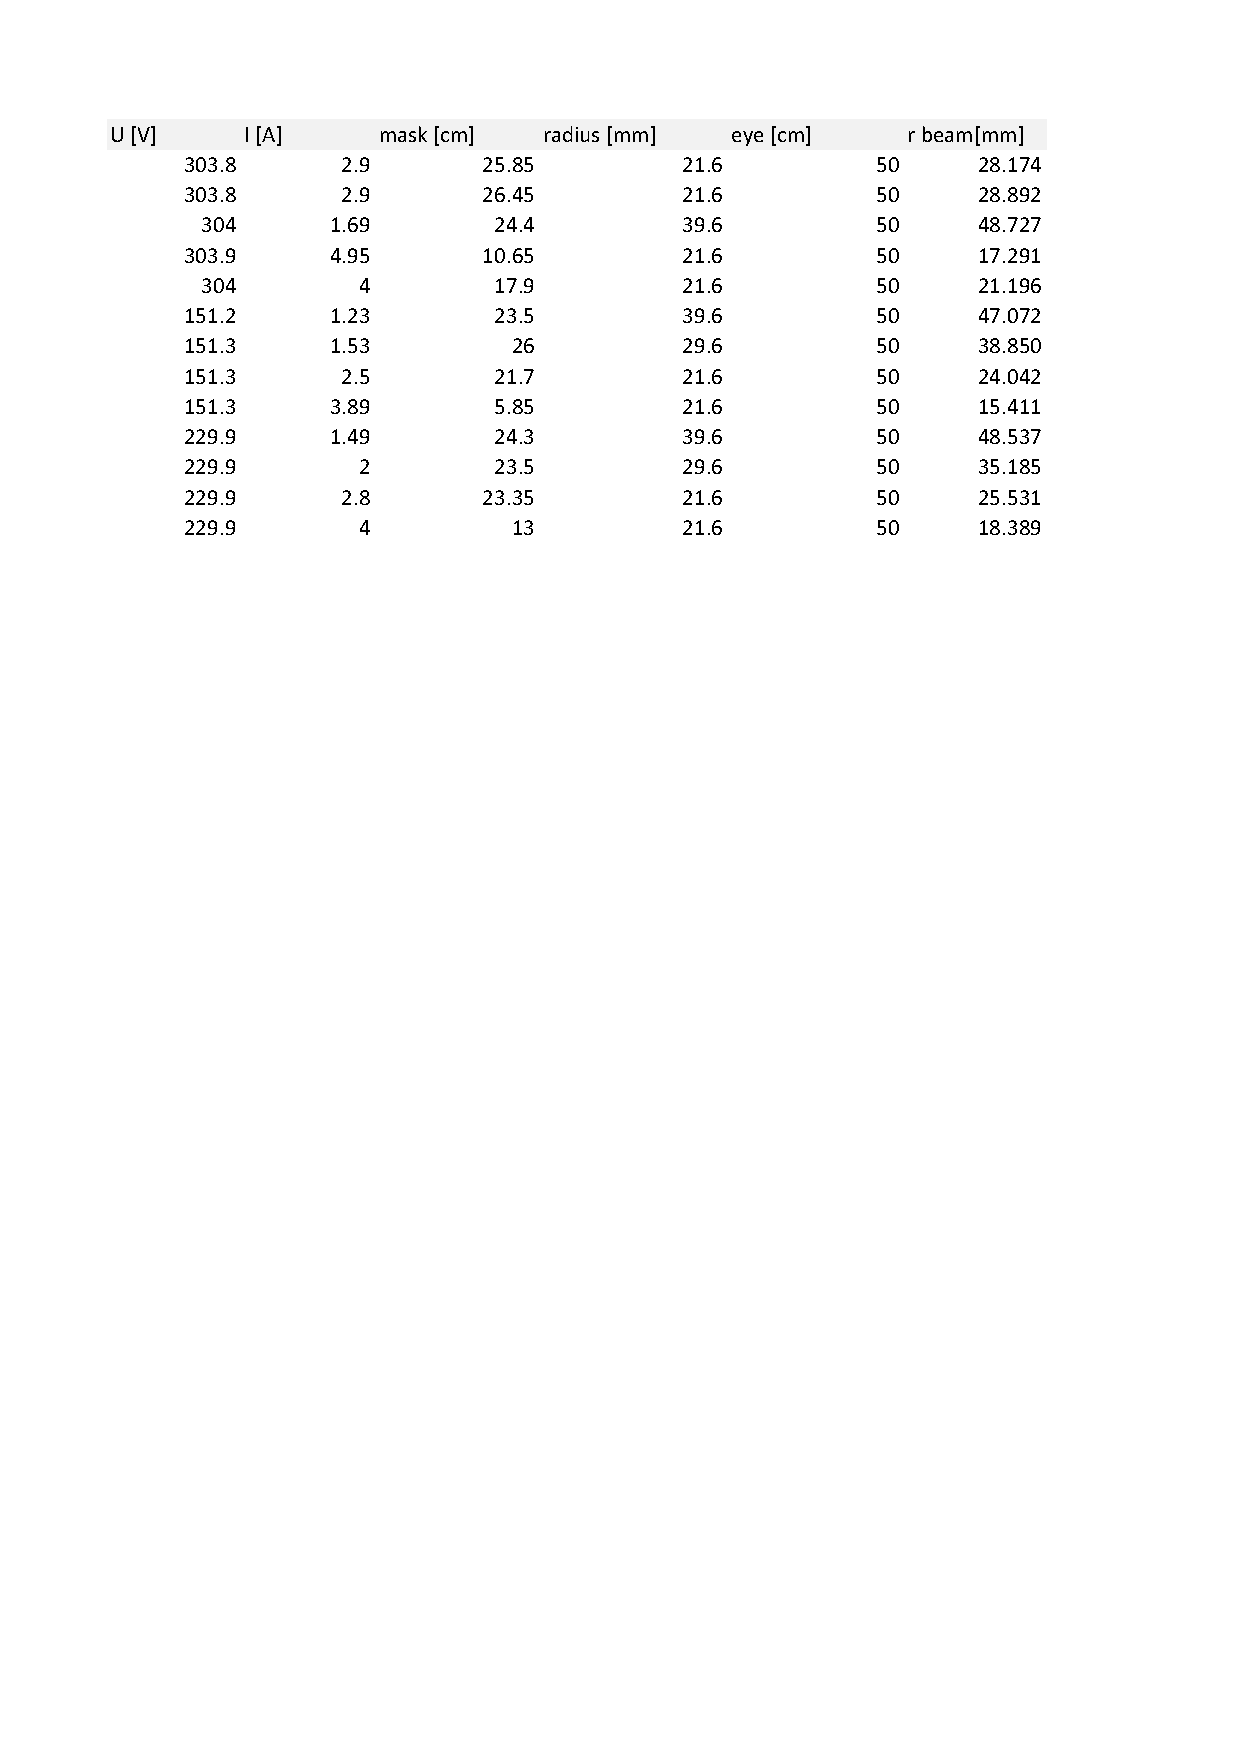
\includegraphics[width=0.9\textwidth]{diag/measurements.pdf}
	\caption{Measured radii $r$ for different values of $U$ and $I$}
	\label{fig:measurements}
\end{figure}

\section{Analysis and Discussion}
Using the theorem of intersecting lines
\begin{equation}
\frac{r}{L	} = \frac{r_{\text{hole}}}{L-l} \Longrightarrow r = \frac{r_{\text{hole}}}{L-l} L
\end{equation}

and all the formula from the theory and error analysis, we deduct the folllowing values:

\begin{table}[H]
\center
\begin{tabular}{|c|c|c|c|c|c|}
\hline
$U$ [$\unit{V}$] & $I$ [$\unit{A}$] & $r$ [$\unit{mm}$] & $r_{\text{theo}}$[$\unit{mm}$] & $e/m \cdot 10^{11} \unit{\frac{coul}{kg}}$ & rel. $\Delta$\\ \hline\hline
$303.8$ & $2.90$ & $28.174 \pm 1.126$ & $27.266$ & $1.647 \pm 0.132$ & $-6.77 \%$\\
$303.8$ & $2.90$ & $28.892 \pm 1.185$ & $27.266$ & $1.566 \pm 0.128$ & $-12.28 \%$\\
$304.0$ & $1.69$ & $48.727 \pm 1.828$ & $46.804$ & $1.623 \pm 0.122$ & $-8.39 \%$\\
$303.9$ & $4.95$ & $17.291 \pm 0.424$ & $15.977$ & $1.502 \pm 0.074$ & $-17.13 \%$\\
$304.0$ & $4.00$ & $21.196 \pm 0.638$ & $19.775$ & $1.531 \pm 0.092$ & $-14.90 \%$\\
$151.2$ & $1.23$ & $47.072 \pm 1.715$ & $45.352$ & $1.633 \pm 0.119$ & $-7.73 \%$\\
$151.3$ & $1.53$ & $38.850 \pm 1.563$ & $36.472$ & $1.550 \pm 0.125$ & $-13.47 \%$\\
$151.3$ & $2.50$ & $24.042 \pm 0.820$ & $22.321$ & $1.516 \pm 0.103$ & $-16.02 \%$\\
$151.3$ & $3.89$ & $15.411 \pm 0.337$ & $14.345$ & $1.524 \pm 0.067$ & $-15.42 \%$\\
$229.9$ & $1.49$ & $48.537 \pm 1.823$ & $46.165$ & $1.591 \pm 0.120$ & $-10.54 \%$\\
$229.9$ & $2.00$ & $35.185 \pm 1.282$ & $34.393$ & $1.681 \pm 0.122$ & $-4.66 \%$\\
$229.9$ & $2.80$ & $25.531 \pm 0.925$ & $24.566$ & $1.628 \pm 0.118$ & $-8.01 \%$\\
$229.9$ & $4.00$ & $18.389 \pm 0.489$ & $17.196$ & $1.538 \pm 0.080$ & $-14.35 \%$\\
\hline
\end{tabular}
\caption{Experiment results with calculated quantities. $r$ and $e/m$ in dependance of $U$ and $I$}
\end{table}

In order to estimate the error of $l$ we measured this quantity twice at the same parameters and we found $s_l = 3 \unit{mm}$\\

As one can see, the errors in the measurement of beam radius $r$ are relatively large and propagate to a large error in the $e/m$ calculation. We expected this to happen and we will discuss this in the ``\nameref{sec:error}'' section.

Summing up, all measurements result in a value for $e/m$ of
\begin{equation}
e/m = \left( 1.579 \pm 0.0161 \right)\cdot 10^{11} \unit{\frac{coul}{kg}}
\end{equation}
which differs from the actual value of 
\begin{equation}
(e/m)_{\text{actual}} = 1.759 \cdot 10^{11} \unit{\frac{coul}{kg}}
\end{equation}
by about $10.21\%$.

\subsection{Sources of error}
\label{sec:error}
Looking for sources of error, we found very few. Both the amperage and the voltage were measured accurately and the measurements showed no reason to doubt that. Errors in the calculation of the strength of the magnetic field can be ruled out, as our documents stated a relative error obtained by using the formulae used being less than $2\%$ \cite[p. 174]{physcript13}. 
The only relevant source of error lies in the measurement of the diameter of the electron beam. We always tried to see the whole beam through the mask, which probably accounts for too large radii. 
\begin{figure}[H]
	\centering
  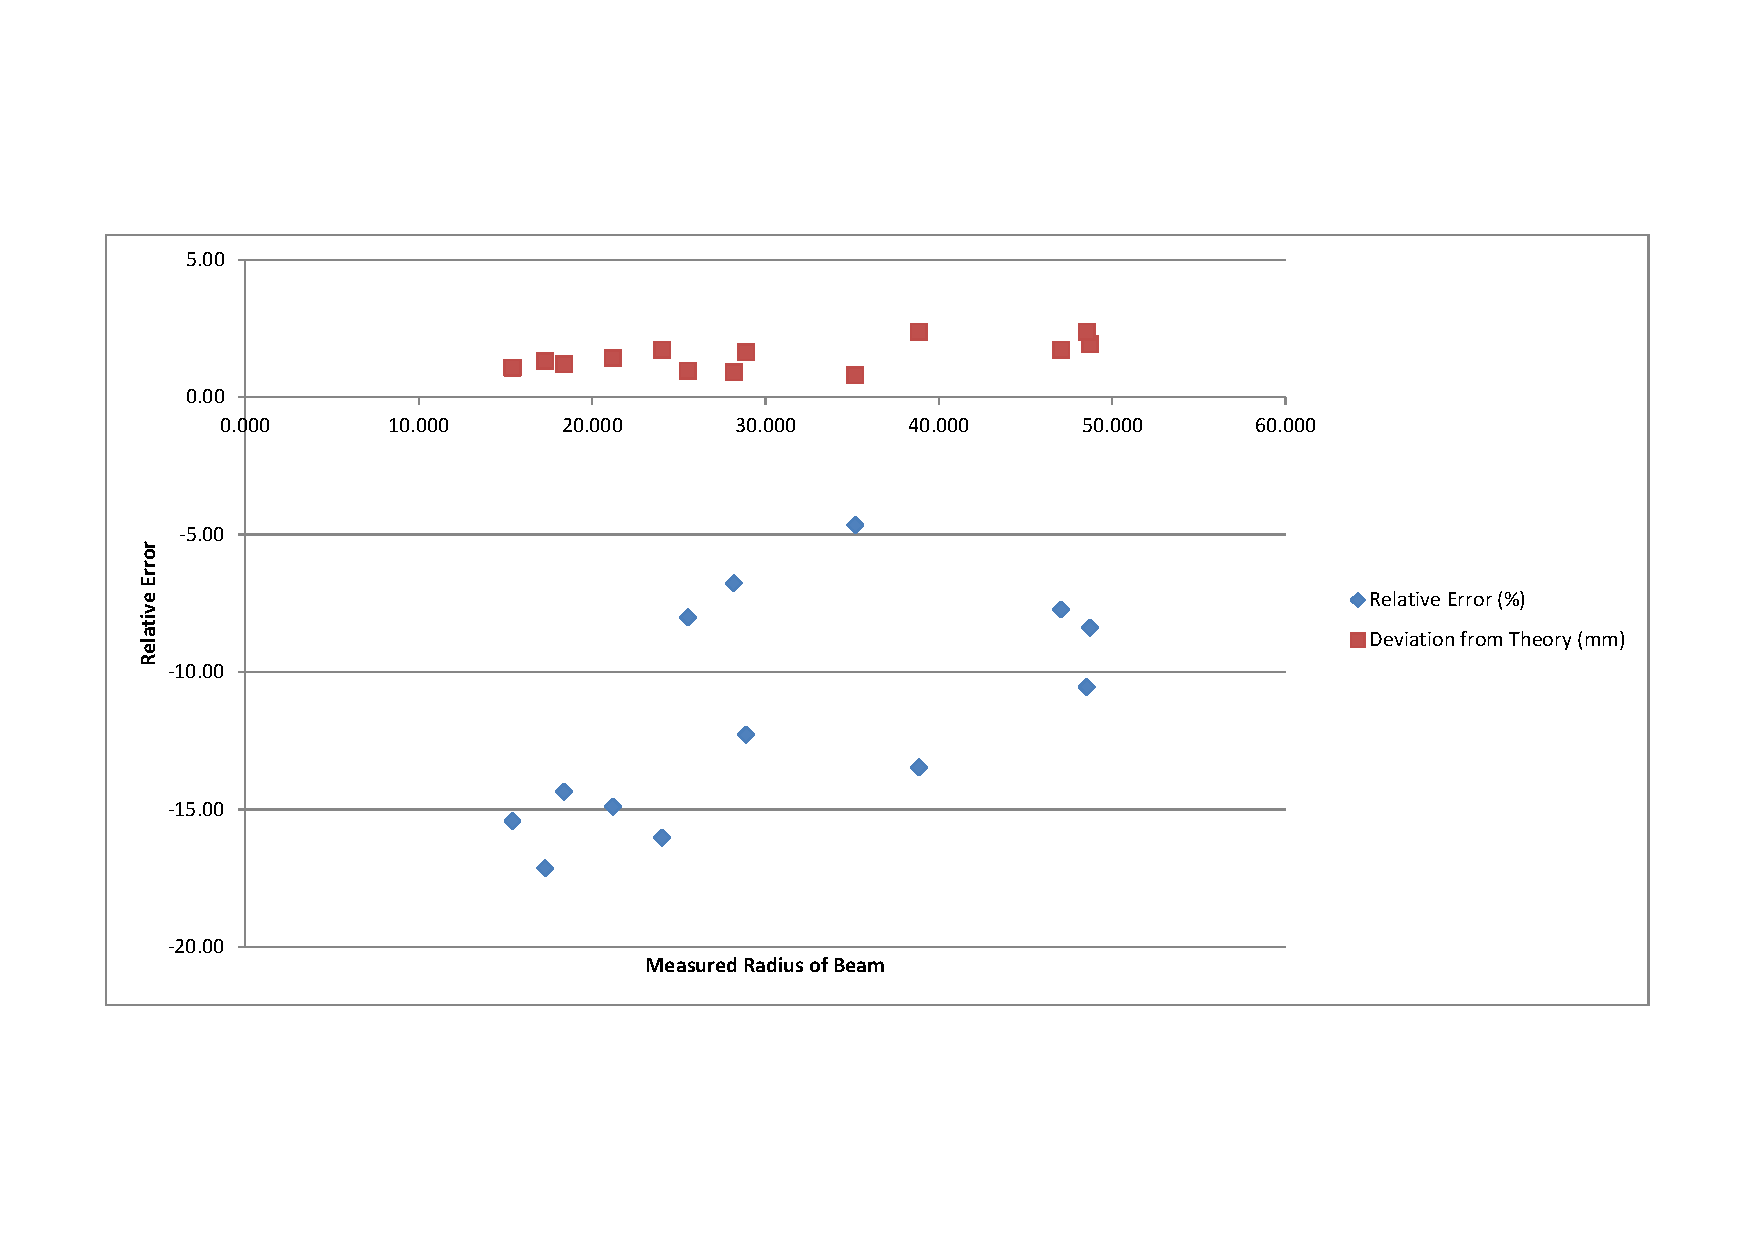
\includegraphics[width=0.9\textwidth]{diag/errors.pdf}
	\caption{Deviation from Theoretical Values for Radii and Relative Error}
	\label{fig:error}
\end{figure}

Looking at \ref{fig:error}, that point can be further supported. The errors for the radii do not see the same order of dependance from the radii as the relative error. A larger measured radius also accounts for our values for the specific electron charge being consistently too low, as a wider circle would mean less charge per mass.

\section{Conclusion}

\begin{thebibliography}{9}

\bibitem{physcript13}
  Peter Wurz,
  \emph{Anleitung zum Physikpraktikum}
  FS2013

\end{thebibliography}

\end{document}
